\documentclass[11pt,]{article}
\usepackage{lmodern}
\usepackage{amssymb,amsmath}
\usepackage{ifxetex,ifluatex}
\usepackage{fixltx2e} % provides \textsubscript
\ifnum 0\ifxetex 1\fi\ifluatex 1\fi=0 % if pdftex
  \usepackage[T1]{fontenc}
  \usepackage[utf8]{inputenc}
\else % if luatex or xelatex
  \ifxetex
    \usepackage{mathspec}
  \else
    \usepackage{fontspec}
  \fi
  \defaultfontfeatures{Ligatures=TeX,Scale=MatchLowercase}
\fi
% use upquote if available, for straight quotes in verbatim environments
\IfFileExists{upquote.sty}{\usepackage{upquote}}{}
% use microtype if available
\IfFileExists{microtype.sty}{%
\usepackage{microtype}
\UseMicrotypeSet[protrusion]{basicmath} % disable protrusion for tt fonts
}{}
\usepackage[margin=1in]{geometry}
\usepackage{hyperref}
\hypersetup{unicode=true,
            pdftitle={Package vars},
            pdfauthor={Paul GUILLOTTE \& Jules CORBEL},
            pdfborder={0 0 0},
            breaklinks=true}
\urlstyle{same}  % don't use monospace font for urls
\usepackage{color}
\usepackage{fancyvrb}
\newcommand{\VerbBar}{|}
\newcommand{\VERB}{\Verb[commandchars=\\\{\}]}
\DefineVerbatimEnvironment{Highlighting}{Verbatim}{commandchars=\\\{\}}
% Add ',fontsize=\small' for more characters per line
\usepackage{framed}
\definecolor{shadecolor}{RGB}{248,248,248}
\newenvironment{Shaded}{\begin{snugshade}}{\end{snugshade}}
\newcommand{\KeywordTok}[1]{\textcolor[rgb]{0.13,0.29,0.53}{\textbf{{#1}}}}
\newcommand{\DataTypeTok}[1]{\textcolor[rgb]{0.13,0.29,0.53}{{#1}}}
\newcommand{\DecValTok}[1]{\textcolor[rgb]{0.00,0.00,0.81}{{#1}}}
\newcommand{\BaseNTok}[1]{\textcolor[rgb]{0.00,0.00,0.81}{{#1}}}
\newcommand{\FloatTok}[1]{\textcolor[rgb]{0.00,0.00,0.81}{{#1}}}
\newcommand{\ConstantTok}[1]{\textcolor[rgb]{0.00,0.00,0.00}{{#1}}}
\newcommand{\CharTok}[1]{\textcolor[rgb]{0.31,0.60,0.02}{{#1}}}
\newcommand{\SpecialCharTok}[1]{\textcolor[rgb]{0.00,0.00,0.00}{{#1}}}
\newcommand{\StringTok}[1]{\textcolor[rgb]{0.31,0.60,0.02}{{#1}}}
\newcommand{\VerbatimStringTok}[1]{\textcolor[rgb]{0.31,0.60,0.02}{{#1}}}
\newcommand{\SpecialStringTok}[1]{\textcolor[rgb]{0.31,0.60,0.02}{{#1}}}
\newcommand{\ImportTok}[1]{{#1}}
\newcommand{\CommentTok}[1]{\textcolor[rgb]{0.56,0.35,0.01}{\textit{{#1}}}}
\newcommand{\DocumentationTok}[1]{\textcolor[rgb]{0.56,0.35,0.01}{\textbf{\textit{{#1}}}}}
\newcommand{\AnnotationTok}[1]{\textcolor[rgb]{0.56,0.35,0.01}{\textbf{\textit{{#1}}}}}
\newcommand{\CommentVarTok}[1]{\textcolor[rgb]{0.56,0.35,0.01}{\textbf{\textit{{#1}}}}}
\newcommand{\OtherTok}[1]{\textcolor[rgb]{0.56,0.35,0.01}{{#1}}}
\newcommand{\FunctionTok}[1]{\textcolor[rgb]{0.00,0.00,0.00}{{#1}}}
\newcommand{\VariableTok}[1]{\textcolor[rgb]{0.00,0.00,0.00}{{#1}}}
\newcommand{\ControlFlowTok}[1]{\textcolor[rgb]{0.13,0.29,0.53}{\textbf{{#1}}}}
\newcommand{\OperatorTok}[1]{\textcolor[rgb]{0.81,0.36,0.00}{\textbf{{#1}}}}
\newcommand{\BuiltInTok}[1]{{#1}}
\newcommand{\ExtensionTok}[1]{{#1}}
\newcommand{\PreprocessorTok}[1]{\textcolor[rgb]{0.56,0.35,0.01}{\textit{{#1}}}}
\newcommand{\AttributeTok}[1]{\textcolor[rgb]{0.77,0.63,0.00}{{#1}}}
\newcommand{\RegionMarkerTok}[1]{{#1}}
\newcommand{\InformationTok}[1]{\textcolor[rgb]{0.56,0.35,0.01}{\textbf{\textit{{#1}}}}}
\newcommand{\WarningTok}[1]{\textcolor[rgb]{0.56,0.35,0.01}{\textbf{\textit{{#1}}}}}
\newcommand{\AlertTok}[1]{\textcolor[rgb]{0.94,0.16,0.16}{{#1}}}
\newcommand{\ErrorTok}[1]{\textcolor[rgb]{0.64,0.00,0.00}{\textbf{{#1}}}}
\newcommand{\NormalTok}[1]{{#1}}
\usepackage{graphicx,grffile}
\makeatletter
\def\maxwidth{\ifdim\Gin@nat@width>\linewidth\linewidth\else\Gin@nat@width\fi}
\def\maxheight{\ifdim\Gin@nat@height>\textheight\textheight\else\Gin@nat@height\fi}
\makeatother
% Scale images if necessary, so that they will not overflow the page
% margins by default, and it is still possible to overwrite the defaults
% using explicit options in \includegraphics[width, height, ...]{}
\setkeys{Gin}{width=\maxwidth,height=\maxheight,keepaspectratio}
\IfFileExists{parskip.sty}{%
\usepackage{parskip}
}{% else
\setlength{\parindent}{0pt}
\setlength{\parskip}{6pt plus 2pt minus 1pt}
}
\setlength{\emergencystretch}{3em}  % prevent overfull lines
\providecommand{\tightlist}{%
  \setlength{\itemsep}{0pt}\setlength{\parskip}{0pt}}
\setcounter{secnumdepth}{0}
% Redefines (sub)paragraphs to behave more like sections
\ifx\paragraph\undefined\else
\let\oldparagraph\paragraph
\renewcommand{\paragraph}[1]{\oldparagraph{#1}\mbox{}}
\fi
\ifx\subparagraph\undefined\else
\let\oldsubparagraph\subparagraph
\renewcommand{\subparagraph}[1]{\oldsubparagraph{#1}\mbox{}}
\fi

%%% Use protect on footnotes to avoid problems with footnotes in titles
\let\rmarkdownfootnote\footnote%
\def\footnote{\protect\rmarkdownfootnote}

%%% Change title format to be more compact
\usepackage{titling}

% Create subtitle command for use in maketitle
\newcommand{\subtitle}[1]{
  \posttitle{
    \begin{center}\large#1\end{center}
    }
}

\setlength{\droptitle}{-2em}

  \title{Package vars}
    \pretitle{\vspace{\droptitle}\centering\huge}
  \posttitle{\par}
    \author{Paul GUILLOTTE \& Jules CORBEL}
    \preauthor{\centering\large\emph}
  \postauthor{\par}
      \predate{\centering\large\emph}
  \postdate{\par}
    \date{01/02/2019}


\begin{document}
\maketitle

{
\setcounter{tocdepth}{2}
\tableofcontents
}
Nous nous intéresserons dans ce document à la mise en place de modèles
VAR afin de prédire la masse salariale trimestrielle. Un modèle VAR,
pour Vecteur AutoRégressif, a pour objectif de capturer les
interdépendances entre les différentes séries temporelles à notre
disposition. Ainsi, chaque variable est expliquée par ses propres
valeurs passées ainsi que par les valeurs passées des autres variables
du modèle.

\section{Visualation des séries}\label{visualation-des-series}

Nous nous intéressons dans cette partie aux différentes séries
trimestrielles à notre disposition. Dans un premier temps, nous nous
intéressons aux corrélations entre les variables deux à deux afin de
nous faire une première idée du lien qu'il existe entre les variables.

\begin{Shaded}
\begin{Highlighting}[]
\NormalTok{trim <-}\StringTok{ }\KeywordTok{read.csv}\NormalTok{(}\StringTok{"~/PFE_Time_Series/Data/Data_Trim.csv"}\NormalTok{, }\DataTypeTok{sep=}\StringTok{";"}\NormalTok{, }\DataTypeTok{dec=}\StringTok{","}\NormalTok{)}
\KeywordTok{corrplot}\NormalTok{(}\KeywordTok{cor}\NormalTok{(trim[}\DecValTok{1}\NormalTok{:}\DecValTok{109}\NormalTok{,-}\DecValTok{1}\NormalTok{]), }\DataTypeTok{method =} \StringTok{"number"}\NormalTok{, }\DataTypeTok{type=}\StringTok{"lower"}\NormalTok{,}
         \DataTypeTok{p.mat=}\KeywordTok{cor.mtest}\NormalTok{(trim[}\DecValTok{1}\NormalTok{:}\DecValTok{109}\NormalTok{,-}\DecValTok{1}\NormalTok{], }\FloatTok{0.95}\NormalTok{)[[}\DecValTok{1}\NormalTok{]], }\DataTypeTok{insig=}\StringTok{"pch"}\NormalTok{,}
         \DataTypeTok{col=}\KeywordTok{colorRampPalette}\NormalTok{(}\KeywordTok{c}\NormalTok{(}\StringTok{"blue"}\NormalTok{, }\StringTok{"light blue"}\NormalTok{, }\StringTok{"red"}\NormalTok{))(}\DecValTok{50}\NormalTok{), }\DataTypeTok{title =} \StringTok{"}
\StringTok{         Corrélations entre les variables trimestrielles"}\NormalTok{)}
\end{Highlighting}
\end{Shaded}

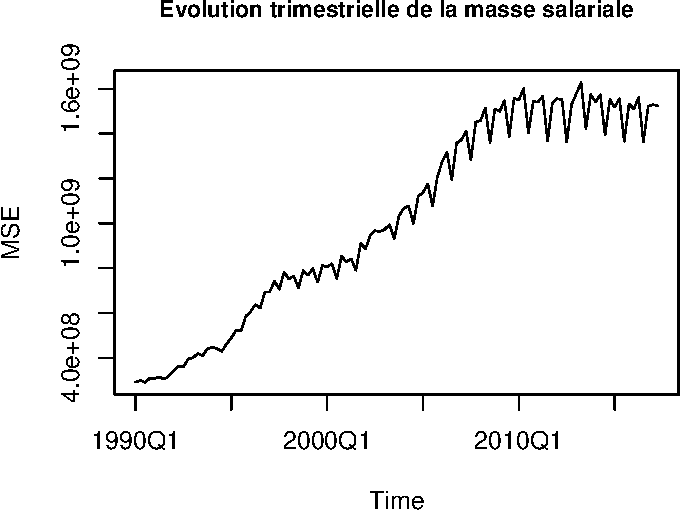
\includegraphics{doc_files/figure-latex/unnamed-chunk-1-1.pdf}

On se rend compte que le taux de chômage des femmes est corrélé
négativement avec toutes les autres variables. Le trio de variables PIB,
masse salariale et SMIC sont extrêmement liées entre elles.

Nous allons maintenant nous attarder sur chaque série individuellement.

\subsection{Masse salariale}\label{masse-salariale}

\begin{Shaded}
\begin{Highlighting}[]
  \NormalTok{MSE <-}\StringTok{ }\KeywordTok{ts}\NormalTok{(trim$MSE, }\DataTypeTok{start =} \DecValTok{1990}\NormalTok{, }\DataTypeTok{end =} \KeywordTok{c}\NormalTok{(}\DecValTok{2017}\NormalTok{, }\DecValTok{2}\NormalTok{), }\DataTypeTok{frequency=}\DecValTok{4}\NormalTok{)}
  \KeywordTok{plot}\NormalTok{(MSE, }\DataTypeTok{main=}\StringTok{"Evolution de la masse salariale trimestrielle"}\NormalTok{)}
\end{Highlighting}
\end{Shaded}

\begin{figure}[htbp]
\centering
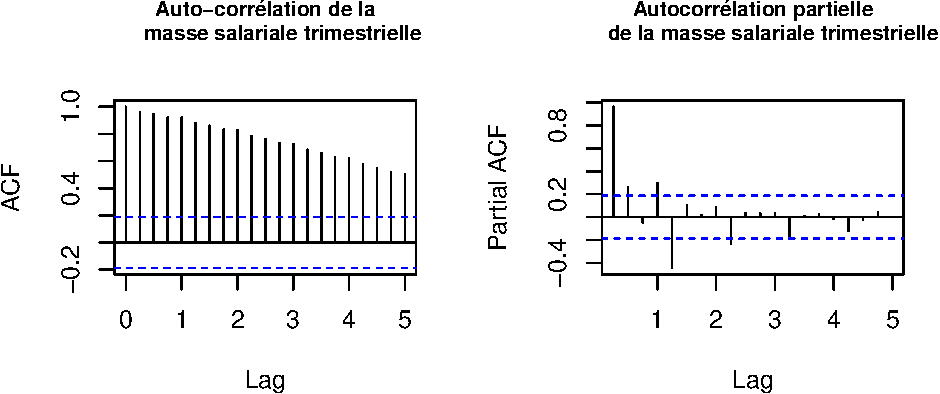
\includegraphics{doc_files/figure-latex/unnamed-chunk-2-1.pdf}
\caption{\label{fig}}
\end{figure}

\begin{Shaded}
\begin{Highlighting}[]
  \KeywordTok{par}\NormalTok{(}\DataTypeTok{mfrow=}\KeywordTok{c}\NormalTok{(}\DecValTok{1}\NormalTok{,}\DecValTok{2}\NormalTok{))}
  \KeywordTok{acf}\NormalTok{(MSE, }\DataTypeTok{main=}\StringTok{"Auto-corrélation de la}
\StringTok{      masse salariale trimestrielle"}\NormalTok{, }\DataTypeTok{lag.max=}\DecValTok{20}\NormalTok{)}
  \KeywordTok{pacf}\NormalTok{(MSE, }\DataTypeTok{main=}\StringTok{"Autocorrélation partielle}
\StringTok{       de la masse trimestrielle"}\NormalTok{, }\DataTypeTok{lag.max=}\DecValTok{20}\NormalTok{)}
\end{Highlighting}
\end{Shaded}

\begin{figure}[htbp]
\centering
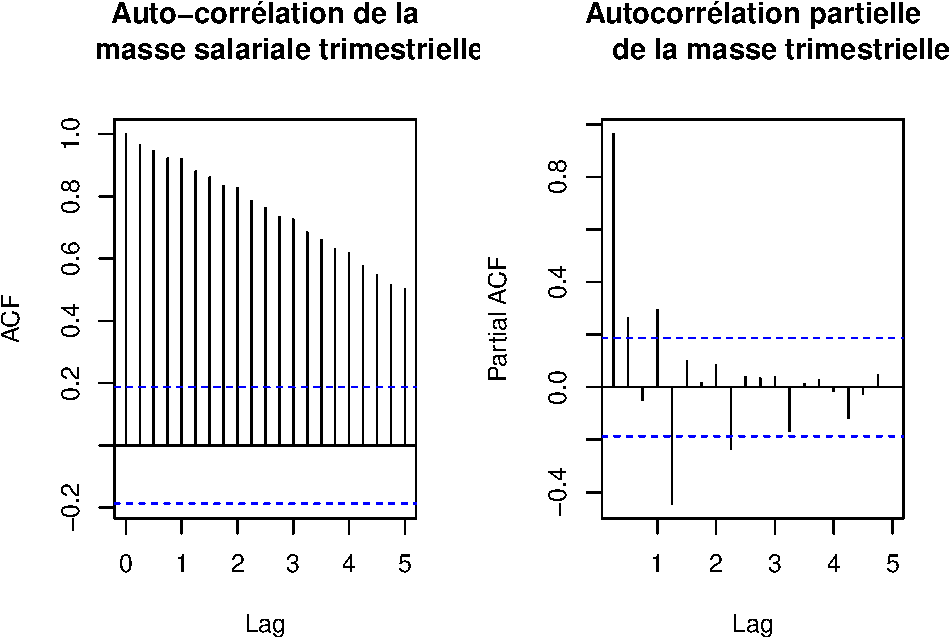
\includegraphics{doc_files/figure-latex/unnamed-chunk-2-2.pdf}
\caption{\label{fig}}
\end{figure}

\begin{Shaded}
\begin{Highlighting}[]
  \KeywordTok{kpss.test}\NormalTok{(MSE)}
\end{Highlighting}
\end{Shaded}

\begin{verbatim}
## Warning in kpss.test(MSE): p-value smaller than printed p-value
\end{verbatim}

\begin{verbatim}
## 
##  KPSS Test for Level Stationarity
## 
## data:  MSE
## KPSS Level = 3.6772, Truncation lag parameter = 2, p-value = 0.01
\end{verbatim}

La masse salariale trimestrielle possède une composante de tendance de
1990 à 2010. La série tend par la suite à stagner. Nous remarquons
également une saisonnalité sur cette série, qui est de plus en plus
marquée à mesure que le temps passe.

Comme la série comporte une tendance et une saisonnalité, elle ne
correspond pas aux deux premières conditions de la stationnarité du
second ordre, soit que la série possède une moyenne et un écart-type
constants. Cela est confirmé par la fonction ACF qui décroît
régulièrement. Nous effectuons également un test de KPSS servant à
vérifier si la série est stationnaire ou non (sous l'hypothèse \(H_{0}\)
la série est stationnaire, et sous l'hypothèse \(H_{1}\) elle ne l'est
pas). La p-value est de 0.01 ce qui nous confirme que la série n'est pas
stationnaire avec un risque de première espèce de 5\%.

\subsection{PIB}\label{pib}

\begin{Shaded}
\begin{Highlighting}[]
  \NormalTok{PIB <-}\StringTok{ }\KeywordTok{ts}\NormalTok{(trim$PIB, }\DataTypeTok{start =} \DecValTok{1990}\NormalTok{, }\DataTypeTok{end =} \KeywordTok{c}\NormalTok{(}\DecValTok{2017}\NormalTok{, }\DecValTok{1}\NormalTok{), }\DataTypeTok{frequency=}\DecValTok{4}\NormalTok{)}
  \KeywordTok{plot}\NormalTok{(PIB, }\DataTypeTok{main=}\StringTok{"Evolution du PIB trimestriel"}\NormalTok{)}
\end{Highlighting}
\end{Shaded}

\begin{figure}[htbp]
\centering
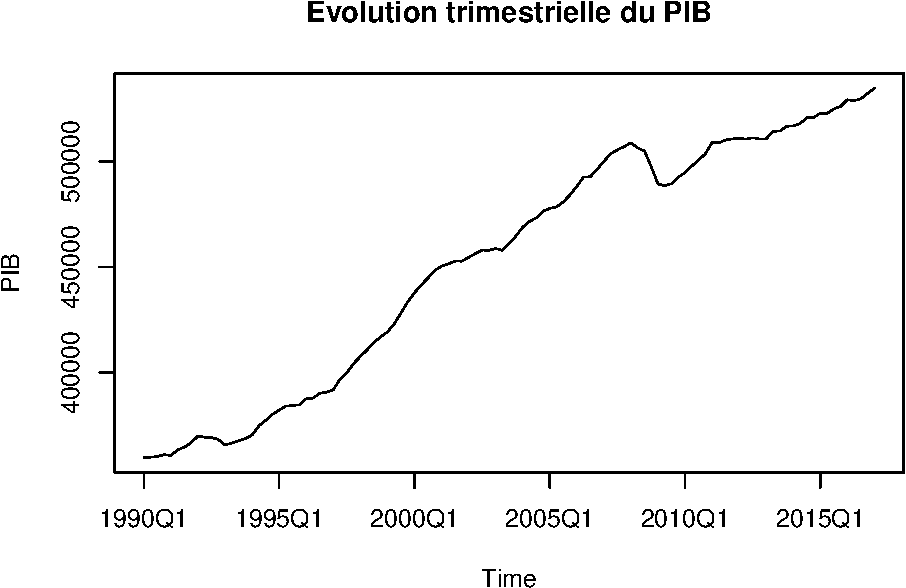
\includegraphics{doc_files/figure-latex/unnamed-chunk-3-1.pdf}
\caption{\label{fig}}
\end{figure}

\begin{Shaded}
\begin{Highlighting}[]
  \KeywordTok{par}\NormalTok{(}\DataTypeTok{mfrow=}\KeywordTok{c}\NormalTok{(}\DecValTok{1}\NormalTok{,}\DecValTok{2}\NormalTok{))}
  \KeywordTok{acf}\NormalTok{(PIB, }\DataTypeTok{main=}\StringTok{"Auto-corrélation }
\StringTok{      du PIB trimestriel"}\NormalTok{, }\DataTypeTok{lag.max=}\DecValTok{20}\NormalTok{)}
  \KeywordTok{pacf}\NormalTok{(PIB, }\DataTypeTok{main=}\StringTok{"Autocorrélation partielle}
\StringTok{       du PIB trimestriel"}\NormalTok{, }\DataTypeTok{lag.max=}\DecValTok{20}\NormalTok{)}
\end{Highlighting}
\end{Shaded}

\begin{figure}[htbp]
\centering
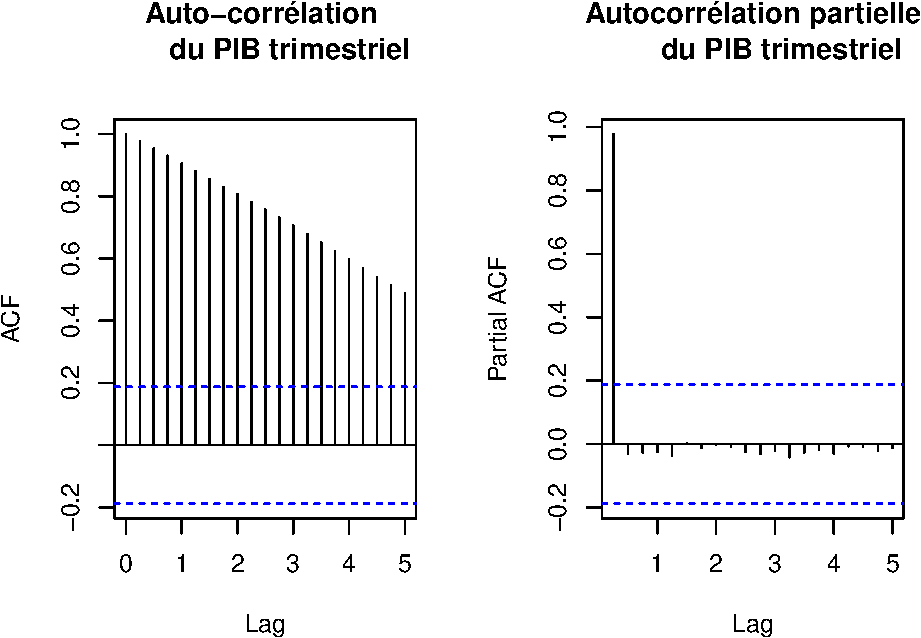
\includegraphics{doc_files/figure-latex/unnamed-chunk-3-2.pdf}
\caption{\label{fig}}
\end{figure}

\begin{Shaded}
\begin{Highlighting}[]
  \KeywordTok{par}\NormalTok{(}\DataTypeTok{mfrow=}\KeywordTok{c}\NormalTok{(}\DecValTok{1}\NormalTok{,}\DecValTok{1}\NormalTok{))}
  \KeywordTok{kpss.test}\NormalTok{(PIB)}
\end{Highlighting}
\end{Shaded}

\begin{verbatim}
## Warning in kpss.test(PIB): p-value smaller than printed p-value
\end{verbatim}

\begin{verbatim}
## 
##  KPSS Test for Level Stationarity
## 
## data:  PIB
## KPSS Level = 3.6473, Truncation lag parameter = 2, p-value = 0.01
\end{verbatim}

Comme pour la masse salariale, le PIB annuel possède une tendance.
Cependant, il ne semble pas posséder de saisonnalité. Cette série n'est
donc pas non plus stationnaire. Nous effectuons à nouveau un test de
KPSS. La p-value est de 0.01 ce qui nous confirme que la série n'est pas
stationnaire avec un risque de première espèce de 5\%.

\subsection{SMIC}\label{smic}

\begin{Shaded}
\begin{Highlighting}[]
  \NormalTok{SMIC <-}\StringTok{ }\KeywordTok{ts}\NormalTok{(trim$SMIC, }\DataTypeTok{start =} \KeywordTok{c}\NormalTok{(}\DecValTok{1990}\NormalTok{,}\DecValTok{1}\NormalTok{), }\DataTypeTok{end =} \KeywordTok{c}\NormalTok{(}\DecValTok{2017}\NormalTok{, }\DecValTok{4}\NormalTok{), }\DataTypeTok{frequency =} \DecValTok{4}\NormalTok{)}
  \KeywordTok{plot}\NormalTok{(SMIC, }\DataTypeTok{main=}\StringTok{"Evolution du SMIC trimestriel"}\NormalTok{)}
\end{Highlighting}
\end{Shaded}

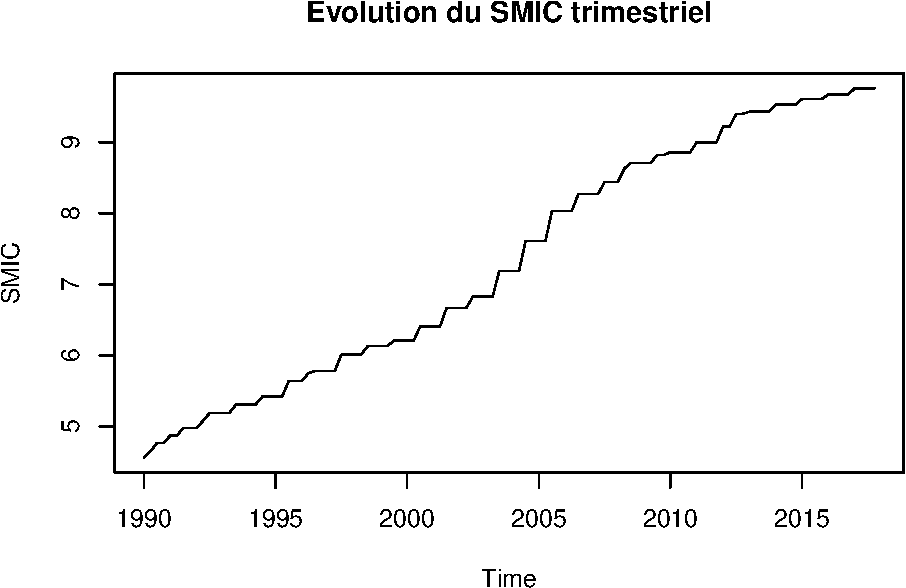
\includegraphics{doc_files/figure-latex/unnamed-chunk-4-1.pdf}

\begin{Shaded}
\begin{Highlighting}[]
  \KeywordTok{par}\NormalTok{(}\DataTypeTok{mfrow=}\KeywordTok{c}\NormalTok{(}\DecValTok{1}\NormalTok{,}\DecValTok{2}\NormalTok{))}
  \KeywordTok{acf}\NormalTok{(SMIC, }\DataTypeTok{main=}\StringTok{"Auto-corrélation du}
\StringTok{      SMIC trimestriel"}\NormalTok{, }\DataTypeTok{lag.max=}\DecValTok{20}\NormalTok{)}
  \KeywordTok{pacf}\NormalTok{(SMIC, }\DataTypeTok{main=}\StringTok{"Autocorrélation partielle}
\StringTok{       du SMIC trimestriel"}\NormalTok{, }\DataTypeTok{lag.max=}\DecValTok{20}\NormalTok{)}
\end{Highlighting}
\end{Shaded}

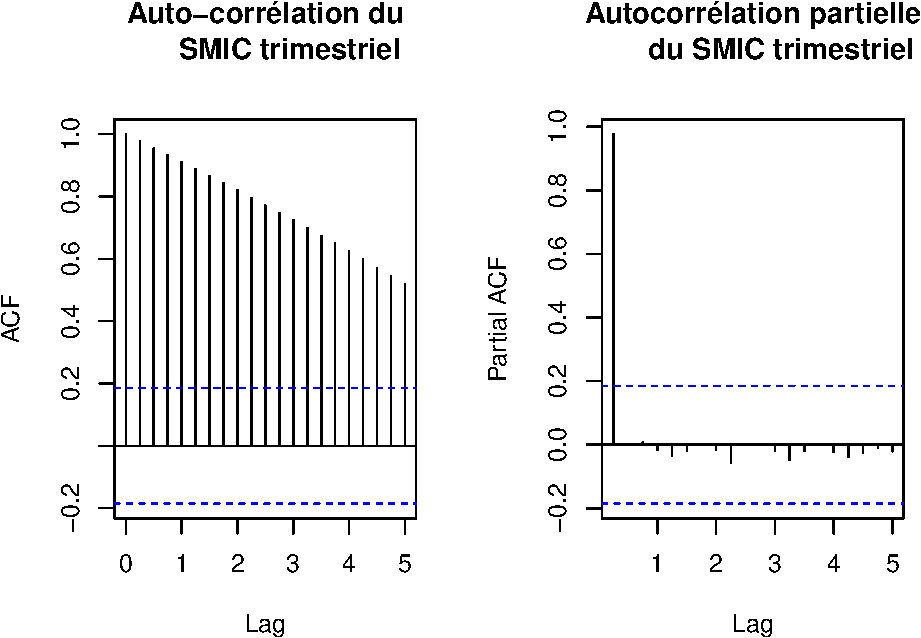
\includegraphics{doc_files/figure-latex/unnamed-chunk-4-2.pdf}

\begin{Shaded}
\begin{Highlighting}[]
  \KeywordTok{par}\NormalTok{(}\DataTypeTok{mfrow=}\KeywordTok{c}\NormalTok{(}\DecValTok{1}\NormalTok{,}\DecValTok{1}\NormalTok{))}
  \KeywordTok{kpss.test}\NormalTok{(SMIC)}
\end{Highlighting}
\end{Shaded}

\begin{verbatim}
## Warning in kpss.test(SMIC): p-value smaller than printed p-value
\end{verbatim}

\begin{verbatim}
## 
##  KPSS Test for Level Stationarity
## 
## data:  SMIC
## KPSS Level = 3.8382, Truncation lag parameter = 2, p-value = 0.01
\end{verbatim}

Au regard de la représentation graphique, on s'aperçoit qu'il y a bien
une tendance. Pour la saisonnalité, il est plus difficile de savoir s'il
en existe une ou pas, puisque la série semble augmenter seulement à
certains temps.

\subsection{Taux de chômage des
femmes}\label{taux-de-chomage-des-femmes}

\begin{Shaded}
\begin{Highlighting}[]
  \NormalTok{TCHOF <-}\StringTok{ }\KeywordTok{ts}\NormalTok{(trim$TCHOF, }\DataTypeTok{start =} \KeywordTok{c}\NormalTok{(}\DecValTok{1990}\NormalTok{,}\DecValTok{1}\NormalTok{), }\DataTypeTok{end =} \KeywordTok{c}\NormalTok{(}\DecValTok{2017}\NormalTok{, }\DecValTok{4}\NormalTok{), }\DataTypeTok{frequency =} \DecValTok{4}\NormalTok{)}
  \KeywordTok{plot}\NormalTok{(TCHOF, }\DataTypeTok{main=}\StringTok{"Evolution du taux de chômage des femmes trimestriel"}\NormalTok{)}
\end{Highlighting}
\end{Shaded}

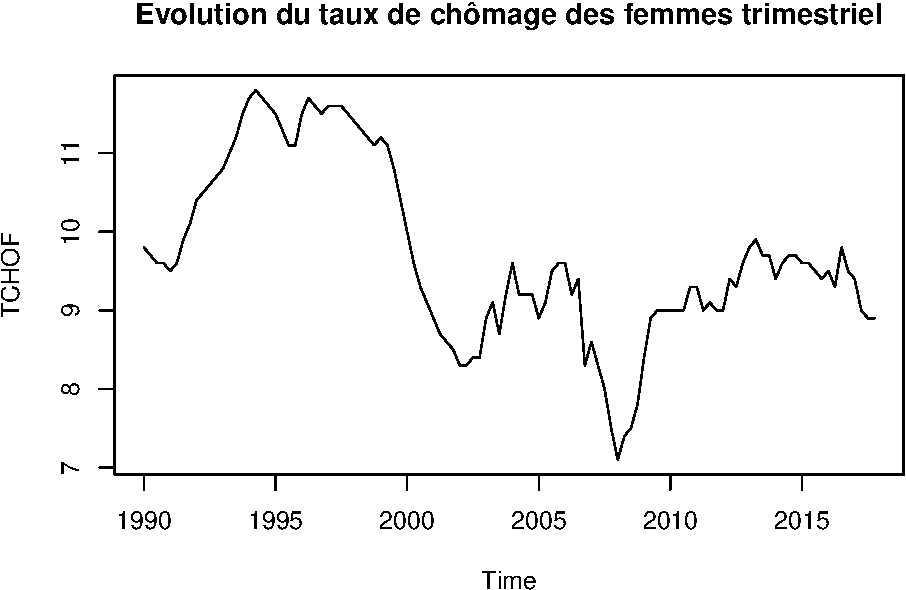
\includegraphics{doc_files/figure-latex/unnamed-chunk-5-1.pdf}

\begin{Shaded}
\begin{Highlighting}[]
  \KeywordTok{par}\NormalTok{(}\DataTypeTok{mfrow=}\KeywordTok{c}\NormalTok{(}\DecValTok{1}\NormalTok{,}\DecValTok{2}\NormalTok{))}
  \KeywordTok{acf}\NormalTok{(TCHOF, }\DataTypeTok{main=}\StringTok{"Auto-corrélation du taux de}
\StringTok{      chômage des femmes trimestriel"}\NormalTok{, }\DataTypeTok{lag.max=}\DecValTok{20}\NormalTok{)}
  \KeywordTok{pacf}\NormalTok{(TCHOF, }\DataTypeTok{main=}\StringTok{"Autocorrélation partielle du}
\StringTok{       taux de chômage des femmes trimestriel"}\NormalTok{, }\DataTypeTok{lag.max=}\DecValTok{20}\NormalTok{)}
\end{Highlighting}
\end{Shaded}

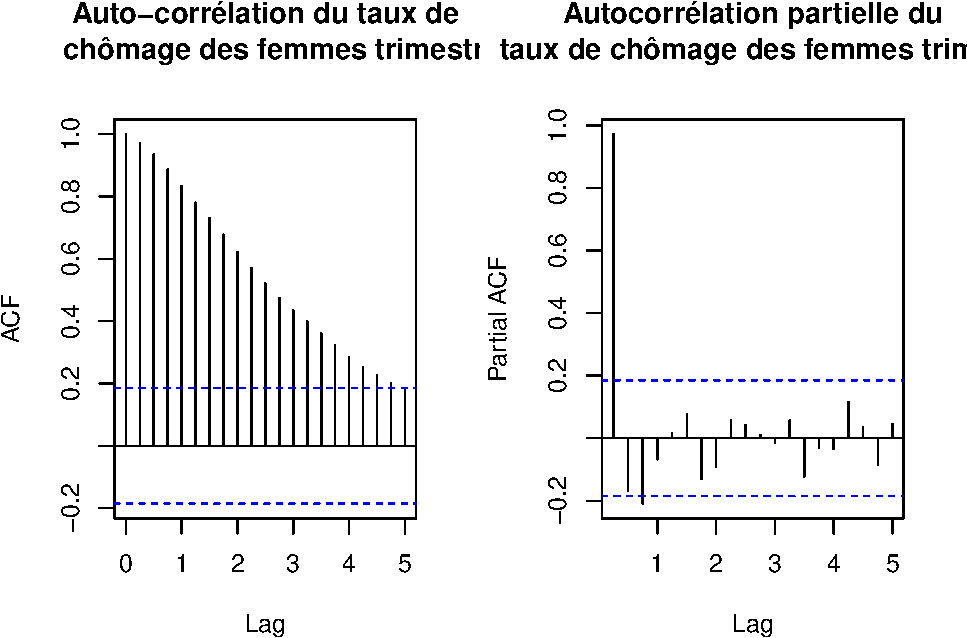
\includegraphics{doc_files/figure-latex/unnamed-chunk-5-2.pdf}

\begin{Shaded}
\begin{Highlighting}[]
  \KeywordTok{par}\NormalTok{(}\DataTypeTok{mfrow=}\KeywordTok{c}\NormalTok{(}\DecValTok{1}\NormalTok{,}\DecValTok{1}\NormalTok{))}
  \KeywordTok{kpss.test}\NormalTok{(TCHOF)}
\end{Highlighting}
\end{Shaded}

\begin{verbatim}
## Warning in kpss.test(TCHOF): p-value smaller than printed p-value
\end{verbatim}

\begin{verbatim}
## 
##  KPSS Test for Level Stationarity
## 
## data:  TCHOF
## KPSS Level = 1.6407, Truncation lag parameter = 2, p-value = 0.01
\end{verbatim}

Pour cette dernière série qui représente le taux de chômage trimestriel
des femmes, il ne semble pas y avoir de saisonnalité. On remarque
cependant qu'il y a bien une tendance. Le test KPSS nous confirme que la
série n'est pas stationnaire.

\section{Transformation des séries}\label{transformation-des-series}

Nous allons maintenant transformer les séries pour les rendre
stationnaires, afin de pouvoir appliquer les différents modèles ensuite.
Afin de stationnariser les séries, nous utiliserons la fonction
decompose qui permet de découper la série en trois : la tendance, la
saisonnalité et les résidus, afin de pouvoir ensuite travailler avec les
résidus.

Pour chacune de ces séries, nous allons créé un échantillon
d'apprentissage, qui nous permettra de construire les différents
modèles, ainsi qu'un échantillon de test, qui nous permettra de comparer
les prédictions des modèles construits avec des vraies valeurs.
L'échantillon d'apprentissage sera composé de toutes les valeurs
jusqu'au 4e trimestre 2015, et celui de test de toutes les valeurs à
partir du 1er trimestre 2016.

\subsection{Masse salariale}\label{masse-salariale-1}

\begin{Shaded}
\begin{Highlighting}[]
  \KeywordTok{plot}\NormalTok{(}\KeywordTok{decompose}\NormalTok{(MSE, }\StringTok{"multiplicative"}\NormalTok{))}
\end{Highlighting}
\end{Shaded}

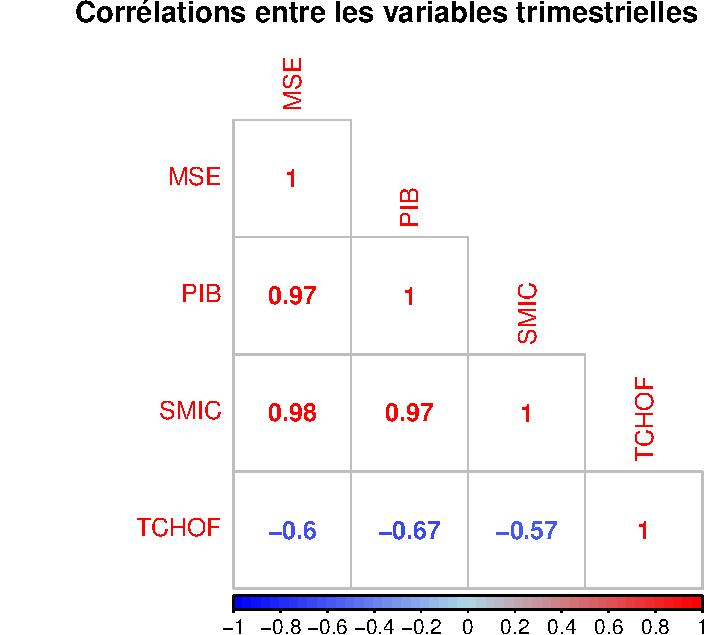
\includegraphics{doc_files/figure-latex/unnamed-chunk-6-1.pdf}

\begin{Shaded}
\begin{Highlighting}[]
  \NormalTok{MSESta <-}\StringTok{ }\KeywordTok{na.omit}\NormalTok{(}\KeywordTok{decompose}\NormalTok{(MSE, }\StringTok{"multiplicative"}\NormalTok{)$random)}
  \NormalTok{MSETrendTest<-}\KeywordTok{window}\NormalTok{(}\KeywordTok{decompose}\NormalTok{(MSE, }\StringTok{"multiplicative"}\NormalTok{)$trend, }\DataTypeTok{start=}\DecValTok{2016}\NormalTok{, }\DataTypeTok{end=}\KeywordTok{c}\NormalTok{(}\DecValTok{2016}\NormalTok{,}\DecValTok{4}\NormalTok{))}
  \NormalTok{MSESeasonalTest<-}\KeywordTok{window}\NormalTok{(}\KeywordTok{decompose}\NormalTok{(MSE, }\StringTok{"multiplicative"}\NormalTok{)$seasonal, }\DataTypeTok{start=}\DecValTok{2016}\NormalTok{, }\DataTypeTok{end=}\KeywordTok{c}\NormalTok{(}\DecValTok{2016}\NormalTok{,}\DecValTok{4}\NormalTok{))}
  \KeywordTok{par}\NormalTok{(}\DataTypeTok{mfrow=}\KeywordTok{c}\NormalTok{(}\DecValTok{1}\NormalTok{,}\DecValTok{2}\NormalTok{))}
  \KeywordTok{acf}\NormalTok{(MSESta, }\DataTypeTok{main=}\StringTok{"Auto-Corrélation de la Masse}
\StringTok{      salariale trimestrielle stationnarisée"}\NormalTok{)}
  \KeywordTok{pacf}\NormalTok{(MSESta, }\DataTypeTok{main=}\StringTok{"Auto-Corrélation partielle de la Masse}
\StringTok{       salariale trimestrielle stationnarisée"}\NormalTok{)}
\end{Highlighting}
\end{Shaded}

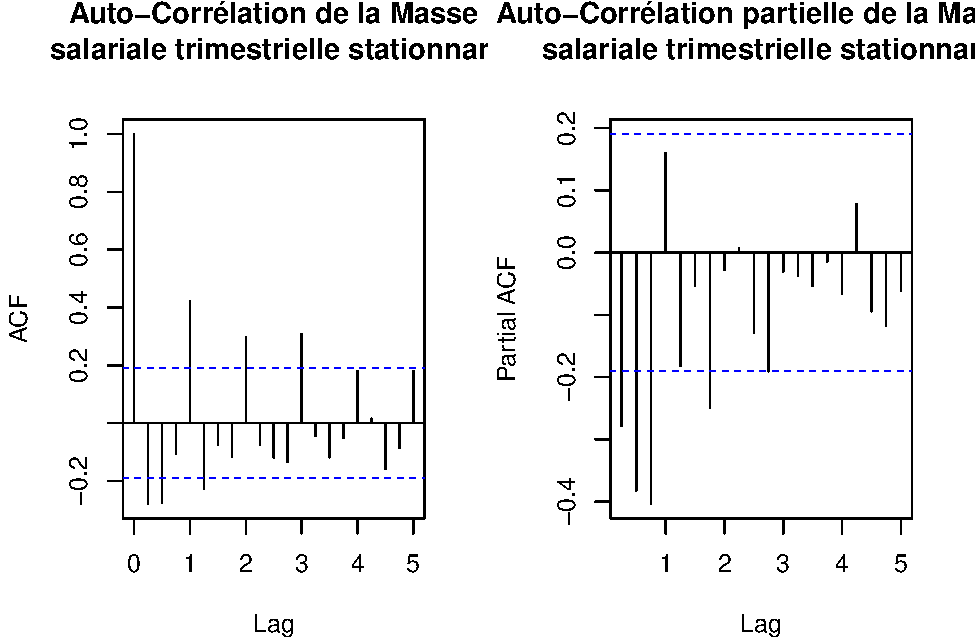
\includegraphics{doc_files/figure-latex/unnamed-chunk-6-2.pdf}

\begin{Shaded}
\begin{Highlighting}[]
  \KeywordTok{par}\NormalTok{(}\DataTypeTok{mfrow=}\KeywordTok{c}\NormalTok{(}\DecValTok{1}\NormalTok{,}\DecValTok{1}\NormalTok{))}
  \KeywordTok{kpss.test}\NormalTok{(MSESta)}
\end{Highlighting}
\end{Shaded}

\begin{verbatim}
## Warning in kpss.test(MSESta): p-value greater than printed p-value
\end{verbatim}

\begin{verbatim}
## 
##  KPSS Test for Level Stationarity
## 
## data:  MSESta
## KPSS Level = 0.021894, Truncation lag parameter = 2, p-value = 0.1
\end{verbatim}

\begin{Shaded}
\begin{Highlighting}[]
  \KeywordTok{plot}\NormalTok{(MSESta, }\DataTypeTok{main=}\StringTok{"Masse salariale trimestrielle stationnarisée"}\NormalTok{)}
\end{Highlighting}
\end{Shaded}

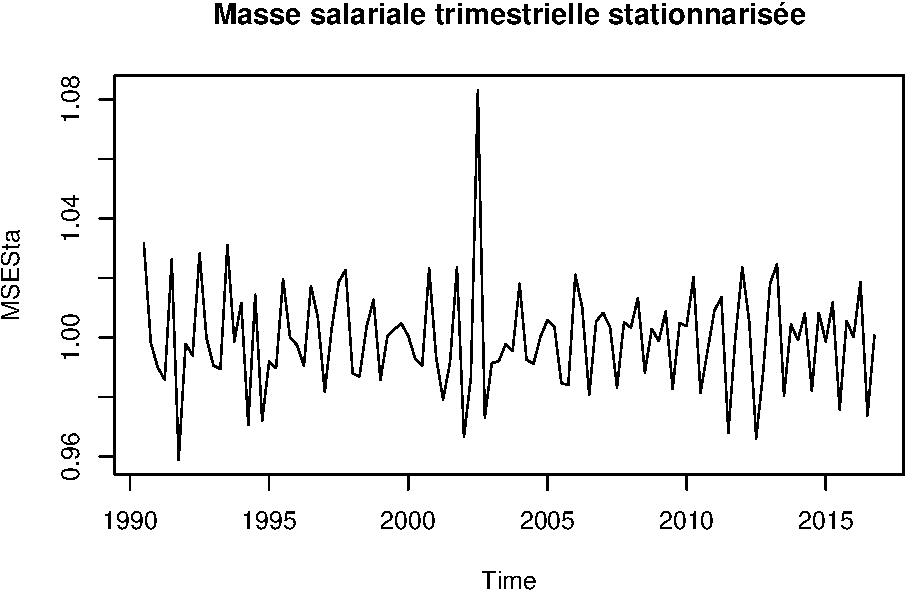
\includegraphics{doc_files/figure-latex/unnamed-chunk-6-3.pdf}

\begin{Shaded}
\begin{Highlighting}[]
  \NormalTok{MSEStaTrain <-}\StringTok{ }\KeywordTok{window}\NormalTok{(MSESta, }\DataTypeTok{end=}\KeywordTok{c}\NormalTok{(}\DecValTok{2015}\NormalTok{,}\DecValTok{4}\NormalTok{))}
  \NormalTok{MSEStaTest <-}\StringTok{ }\KeywordTok{window}\NormalTok{(MSESta, }\DataTypeTok{start=}\DecValTok{2016}\NormalTok{)}
  \NormalTok{MSETrain <-}\StringTok{ }\KeywordTok{window}\NormalTok{(MSE, }\DataTypeTok{end=}\KeywordTok{c}\NormalTok{(}\DecValTok{2015}\NormalTok{,}\DecValTok{4}\NormalTok{))}
  \NormalTok{MSETest <-}\StringTok{ }\KeywordTok{window}\NormalTok{(MSE, }\DataTypeTok{start=}\DecValTok{2016}\NormalTok{)}
\end{Highlighting}
\end{Shaded}

Nous nous intéressons aux ACF, PACF et test de KPSS afin de vérifier si
les résidus obtenus à l'aide de la fonction decompose sont
stationnaires. Bien que l'ACF et la PACF nous mettent en garde d'une
possible non stationnarité de la série, la p-value du test de KPSS nous
amène à conserver l'hypothèse de stationnarité de la série avec un seuil
de confiance à 5\%.

\subsection{PIB}\label{pib-1}

\begin{Shaded}
\begin{Highlighting}[]
  \NormalTok{PIBSta <-}\StringTok{ }\KeywordTok{na.omit}\NormalTok{(}\KeywordTok{decompose}\NormalTok{(PIB, }\StringTok{"multiplicative"}\NormalTok{)$random)}
  \KeywordTok{par}\NormalTok{(}\DataTypeTok{mfrow=}\KeywordTok{c}\NormalTok{(}\DecValTok{1}\NormalTok{,}\DecValTok{2}\NormalTok{))}
  \KeywordTok{acf}\NormalTok{(PIBSta, }\DataTypeTok{main=}\StringTok{"Auto-Corrélation du PIB}
\StringTok{      trimestrielle stationnarisée"}\NormalTok{)}
  \KeywordTok{pacf}\NormalTok{(PIBSta, }\DataTypeTok{main=}\StringTok{"Auto-Corrélation partielle du PIB}
\StringTok{      trimestrielle stationnarisée"}\NormalTok{)}
\end{Highlighting}
\end{Shaded}

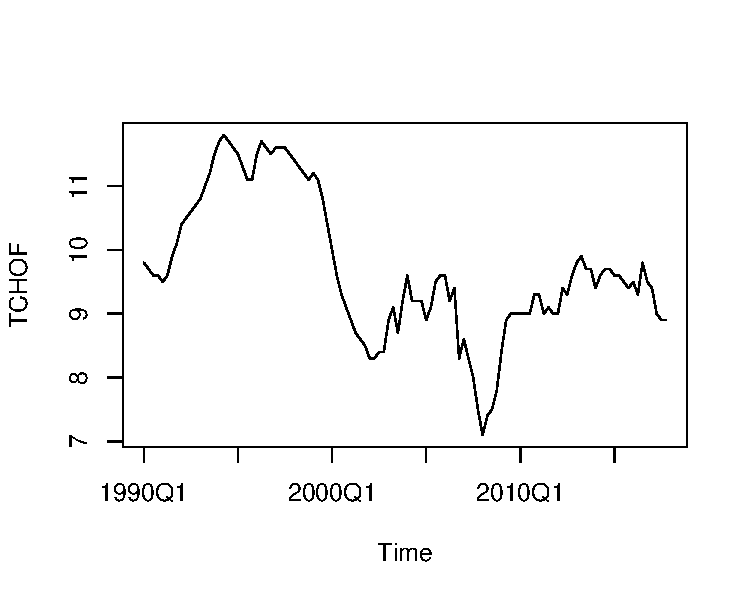
\includegraphics{doc_files/figure-latex/unnamed-chunk-7-1.pdf}

\begin{Shaded}
\begin{Highlighting}[]
  \KeywordTok{par}\NormalTok{(}\DataTypeTok{mfrow=}\KeywordTok{c}\NormalTok{(}\DecValTok{1}\NormalTok{,}\DecValTok{1}\NormalTok{))}
  \KeywordTok{kpss.test}\NormalTok{(PIBSta)}
\end{Highlighting}
\end{Shaded}

\begin{verbatim}
## Warning in kpss.test(PIBSta): p-value greater than printed p-value
\end{verbatim}

\begin{verbatim}
## 
##  KPSS Test for Level Stationarity
## 
## data:  PIBSta
## KPSS Level = 0.024935, Truncation lag parameter = 2, p-value = 0.1
\end{verbatim}

\begin{Shaded}
\begin{Highlighting}[]
  \KeywordTok{plot}\NormalTok{(PIBSta, }\DataTypeTok{main=}\StringTok{"PIB trimestriel stationnarisé"}\NormalTok{)}
\end{Highlighting}
\end{Shaded}

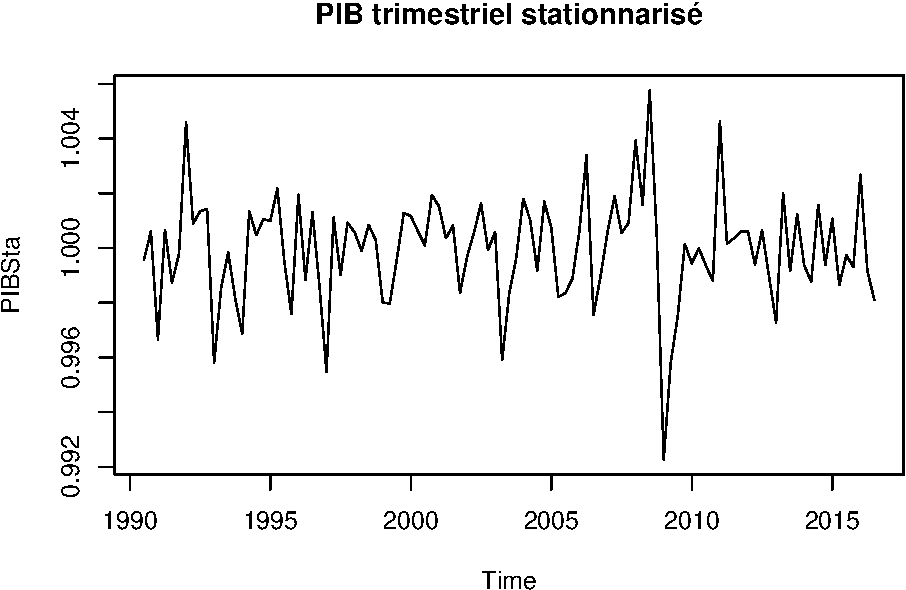
\includegraphics{doc_files/figure-latex/unnamed-chunk-7-2.pdf}

\begin{Shaded}
\begin{Highlighting}[]
  \NormalTok{PIBStaTrain <-}\StringTok{ }\KeywordTok{window}\NormalTok{(PIBSta, }\DataTypeTok{end=}\KeywordTok{c}\NormalTok{(}\DecValTok{2015}\NormalTok{,}\DecValTok{4}\NormalTok{))}
  \NormalTok{PIBStaTest <-}\StringTok{ }\KeywordTok{window}\NormalTok{(PIBSta, }\DataTypeTok{start=}\DecValTok{2016}\NormalTok{)}
  \NormalTok{PIBTrain <-}\StringTok{ }\KeywordTok{window}\NormalTok{(PIB, }\DataTypeTok{end=}\KeywordTok{c}\NormalTok{(}\DecValTok{2015}\NormalTok{,}\DecValTok{4}\NormalTok{))}
  \NormalTok{PIBTest <-}\StringTok{ }\KeywordTok{window}\NormalTok{(PIB, }\DataTypeTok{start=}\DecValTok{2016}\NormalTok{)}
\end{Highlighting}
\end{Shaded}

Nous nous intéressons aux ACF, PACF et test de KPSS afin de vérifier si
les résidus obtenus à l'aide de la fonction decompose sont
stationnaires. Au regard de ces différentes informations, nous pouvons
conclure à la stationnarité des résidus.

\subsection{SMIC}\label{smic-1}

\begin{Shaded}
\begin{Highlighting}[]
  \NormalTok{SMICSta <-}\StringTok{ }\KeywordTok{na.omit}\NormalTok{(}\KeywordTok{decompose}\NormalTok{(SMIC)$random)}
  \KeywordTok{par}\NormalTok{(}\DataTypeTok{mfrow=}\KeywordTok{c}\NormalTok{(}\DecValTok{1}\NormalTok{,}\DecValTok{2}\NormalTok{))}
  \KeywordTok{acf}\NormalTok{(SMICSta, }\DataTypeTok{main=}\StringTok{"Auto-Corrélation du SMIC}
\StringTok{      trimestrielle stationnarisée"}\NormalTok{)}
  \KeywordTok{pacf}\NormalTok{(SMICSta, }\DataTypeTok{main=}\StringTok{"Auto-Corrélation partielle du SMIC}
\StringTok{      trimestrielle stationnarisée"}\NormalTok{)}
\end{Highlighting}
\end{Shaded}

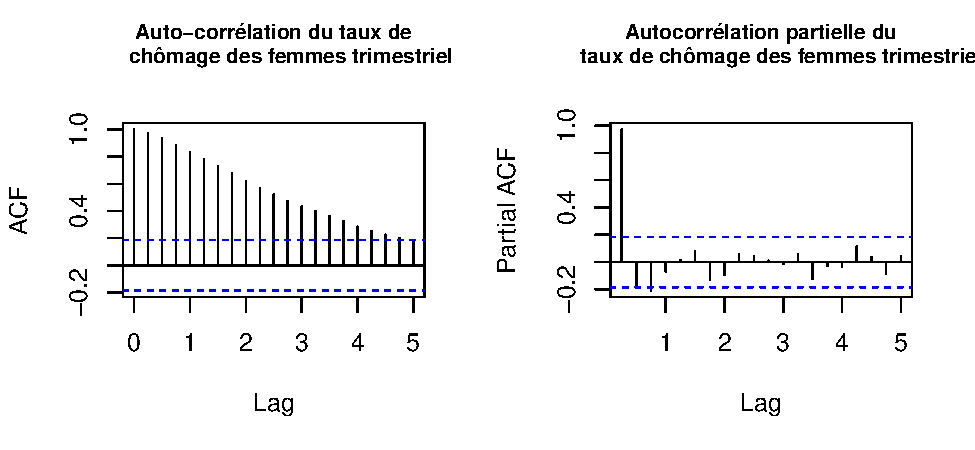
\includegraphics{doc_files/figure-latex/unnamed-chunk-8-1.pdf}

\begin{Shaded}
\begin{Highlighting}[]
  \KeywordTok{par}\NormalTok{(}\DataTypeTok{mfrow=}\KeywordTok{c}\NormalTok{(}\DecValTok{1}\NormalTok{,}\DecValTok{1}\NormalTok{))}
  \KeywordTok{kpss.test}\NormalTok{(SMICSta)}
\end{Highlighting}
\end{Shaded}

\begin{verbatim}
## Warning in kpss.test(SMICSta): p-value greater than printed p-value
\end{verbatim}

\begin{verbatim}
## 
##  KPSS Test for Level Stationarity
## 
## data:  SMICSta
## KPSS Level = 0.034306, Truncation lag parameter = 2, p-value = 0.1
\end{verbatim}

\begin{Shaded}
\begin{Highlighting}[]
  \KeywordTok{plot}\NormalTok{(SMICSta, }\DataTypeTok{main=}\StringTok{"SMIC trimestriel stationnarisé"}\NormalTok{)}
\end{Highlighting}
\end{Shaded}

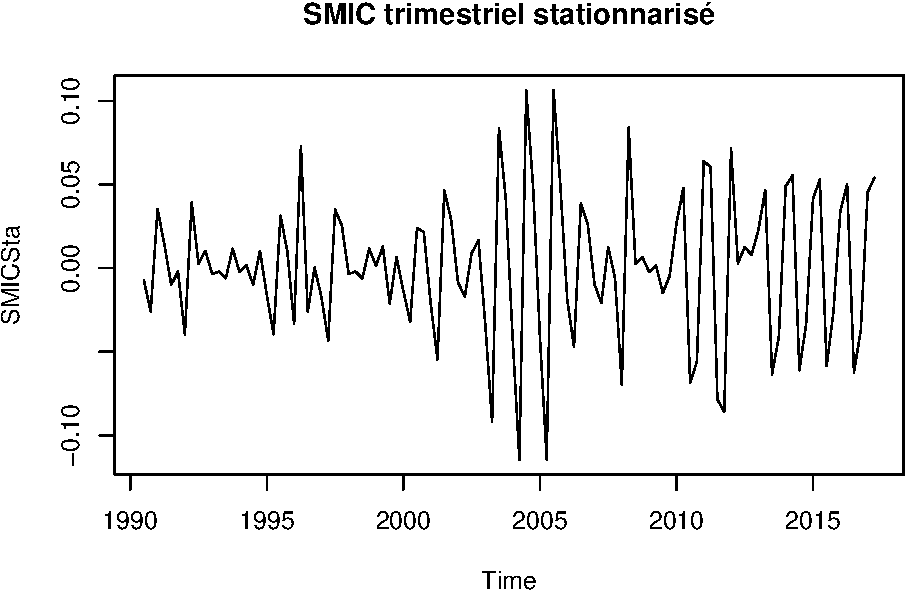
\includegraphics{doc_files/figure-latex/unnamed-chunk-8-2.pdf}

\begin{Shaded}
\begin{Highlighting}[]
  \NormalTok{SMICStaTrain <-}\StringTok{ }\KeywordTok{window}\NormalTok{(SMICSta, }\DataTypeTok{end=}\KeywordTok{c}\NormalTok{(}\DecValTok{2015}\NormalTok{,}\DecValTok{4}\NormalTok{))}
  \NormalTok{SMICStaTest <-}\StringTok{ }\KeywordTok{window}\NormalTok{(SMICSta, }\DataTypeTok{start=}\DecValTok{2016}\NormalTok{)}
  \NormalTok{SMICTrain <-}\StringTok{ }\KeywordTok{window}\NormalTok{(SMIC, }\DataTypeTok{end=}\KeywordTok{c}\NormalTok{(}\DecValTok{2015}\NormalTok{,}\DecValTok{4}\NormalTok{))}
  \NormalTok{SMICTest <-}\StringTok{ }\KeywordTok{window}\NormalTok{(SMIC, }\DataTypeTok{start=}\DecValTok{2016}\NormalTok{)}
\end{Highlighting}
\end{Shaded}

Comme pour la masse salariale, les ACF et PACF semblent montrer que la
série résiduelle pourrait ne pas être stationnaire. Cependant le test de
KPSS nous permet de conserver l'hypothèse de stationnarité des résidus.

\subsection{Taux de chômage des
femmes}\label{taux-de-chomage-des-femmes-1}

\begin{Shaded}
\begin{Highlighting}[]
  \NormalTok{TCHOFSta <-}\StringTok{ }\KeywordTok{na.omit}\NormalTok{(}\KeywordTok{decompose}\NormalTok{(TCHOF)$random)}
  \KeywordTok{par}\NormalTok{(}\DataTypeTok{mfrow=}\KeywordTok{c}\NormalTok{(}\DecValTok{1}\NormalTok{,}\DecValTok{2}\NormalTok{))}
  \KeywordTok{acf}\NormalTok{(TCHOFSta, }\DataTypeTok{main=}\StringTok{"Auto-Corrélation du Taux de}
\StringTok{      chômage des femmes}
\StringTok{      trimestrielle stationnarisée"}\NormalTok{)}
  \KeywordTok{pacf}\NormalTok{(TCHOFSta, }\DataTypeTok{main=}\StringTok{"Auto-Corrélation partielle}
\StringTok{      du Taux de chômage des femmes}
\StringTok{      trimestrielle stationnarisée"}\NormalTok{)}
\end{Highlighting}
\end{Shaded}

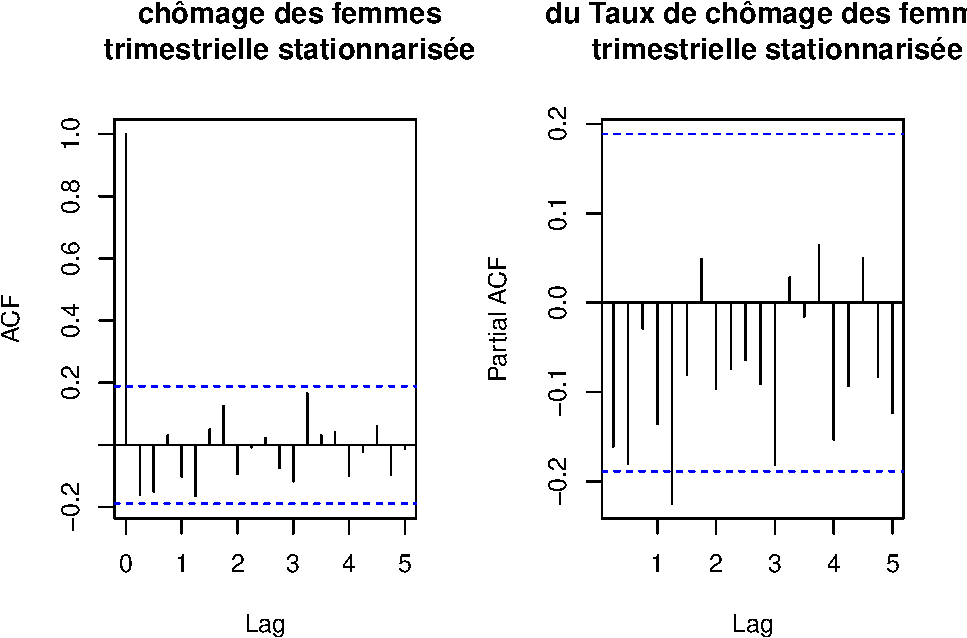
\includegraphics{doc_files/figure-latex/unnamed-chunk-9-1.pdf}

\begin{Shaded}
\begin{Highlighting}[]
  \KeywordTok{par}\NormalTok{(}\DataTypeTok{mfrow=}\KeywordTok{c}\NormalTok{(}\DecValTok{1}\NormalTok{,}\DecValTok{1}\NormalTok{))}
  \KeywordTok{kpss.test}\NormalTok{(TCHOFSta)}
\end{Highlighting}
\end{Shaded}

\begin{verbatim}
## Warning in kpss.test(TCHOFSta): p-value greater than printed p-value
\end{verbatim}

\begin{verbatim}
## 
##  KPSS Test for Level Stationarity
## 
## data:  TCHOFSta
## KPSS Level = 0.02222, Truncation lag parameter = 2, p-value = 0.1
\end{verbatim}

\begin{Shaded}
\begin{Highlighting}[]
  \KeywordTok{plot}\NormalTok{(TCHOFSta, }\DataTypeTok{main=}\StringTok{"Taux de chômage trimestriel des femmes stationnarisé"}\NormalTok{)}
\end{Highlighting}
\end{Shaded}

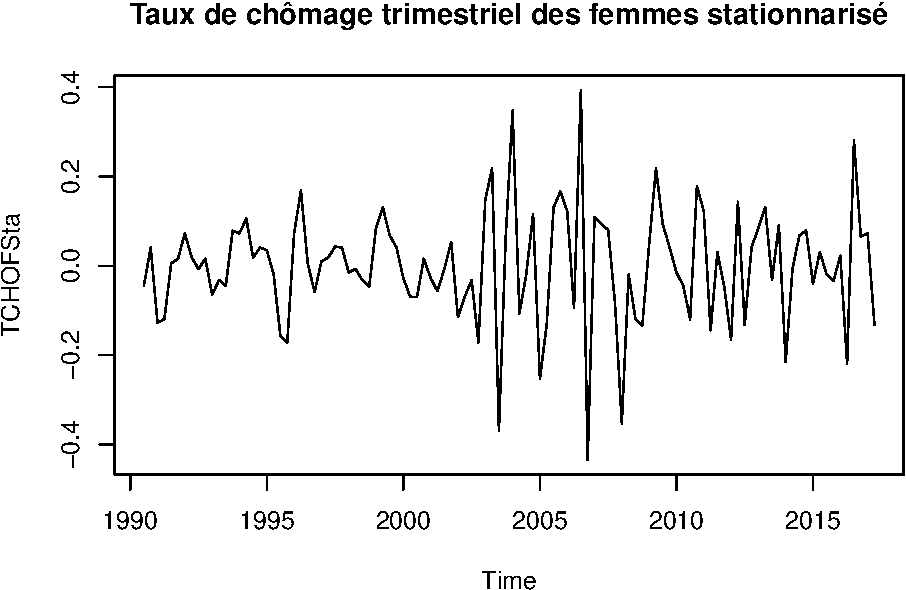
\includegraphics{doc_files/figure-latex/unnamed-chunk-9-2.pdf}

\begin{Shaded}
\begin{Highlighting}[]
  \NormalTok{TCHOFStaTrain <-}\StringTok{ }\KeywordTok{window}\NormalTok{(TCHOFSta, }\DataTypeTok{end=}\KeywordTok{c}\NormalTok{(}\DecValTok{2015}\NormalTok{,}\DecValTok{4}\NormalTok{))}
  \NormalTok{TCHOFStaTest <-}\StringTok{ }\KeywordTok{window}\NormalTok{(TCHOFSta, }\DataTypeTok{start=}\DecValTok{2016}\NormalTok{)}
  \NormalTok{TCHOFTrain <-}\StringTok{ }\KeywordTok{window}\NormalTok{(TCHOF, }\DataTypeTok{end=}\KeywordTok{c}\NormalTok{(}\DecValTok{2015}\NormalTok{,}\DecValTok{4}\NormalTok{))}
  \NormalTok{TCHOFTest <-}\StringTok{ }\KeywordTok{window}\NormalTok{(TCHOF, }\DataTypeTok{start=}\DecValTok{2016}\NormalTok{)}
\end{Highlighting}
\end{Shaded}

En ce qui concerne le taux de chômage des femmes, en regardant l'ACF,
PACF et le test de KPSS, on peut conclure que la série résiduelle est
stationnaire.

Maintenant que toutes les séries ont été stationnarisées, nous allons
pouvoir construire des modèles VAR.

\section{Calcul de l'ordre p}\label{calcul-de-lordre-p}

Afin de mettre en place une modélisation VAR, nous devons dans un
premier temps nous intéresser à l'ordre p du modèle VAR. L'ordre p
correspond à l'ordre de l'opérateur de retard, c'est-à-dire le nombre de
valeurs du passé qui ont un impact sur la valeur à un instant défini.
Dans le package \textbf{vars}, la fonction VARselect permet de
déterminer les valeurs de 4 critères (AIC, HQ, SC et FPE) pour
différentes valeurs de l'ordre p.

Pour les critères suivants, n correspond à l'ordre de différenciation, T
le nombre d'observations et K le nombre de variables et
\(\tilde{\Sigma}_u (n) = T^{-1} \Sigma_{t=1}^T \hat{u}_t \hat{u}_t'\).

Le critère AIC (Aikaike information criterion) se calcule, dans ce
package, de la manière suivante :
\(AIC(n) = \ln \det(\tilde{\Sigma}_u(n)) + \frac{2}{T}n K^2 \quad\).
L'objectif est de minimiser ce critère.

Le critère HQ (Hannan-Quinn criterion) se calcule, dans ce package, de
la manière suivante :
\(HQ(n) = \ln \det(\tilde{\Sigma}_u(n)) + \frac{2 \ln(\ln(T))}{T}n K^2 \quad\).
L'objectif est de minimiser ce critère. Contrairement à l'AIC, ce
critère n'est pas asymptotiquement efficace.

Le critère SC (Schwarz criterion) se calcule dans ce package de la
manière suivante :
\(SC(n) = \ln \det(\tilde{\Sigma}_u(n)) + \frac{\ln(T)}{T}n K^2 \quad\).
L'objectif est de minimiser ce critère. Ce critère est équivalent au
BIC.`

Le dernier critère, le critère FPE (Final Prediction Error), est un
critère à minimiser. Cependant nous ne comprenons pas son
fonctionnement. Nous ne l'utiliserons donc pas.

Dans cette partie, nous développerons le fonctionement de la
méthodologie en l'appliquant uniquement au modèle complet, soit celui
prenant en compte les variables PIB, SMIC et taux de chômage des femmes.

\begin{Shaded}
\begin{Highlighting}[]
\NormalTok{selec <-}\StringTok{ }\KeywordTok{VARselect}\NormalTok{(}\KeywordTok{cbind}\NormalTok{(MSEStaTrain, PIBStaTrain, SMICStaTrain, TCHOFStaTrain), }\DataTypeTok{lag.max=}\DecValTok{10}\NormalTok{)}
\KeywordTok{par}\NormalTok{(}\DataTypeTok{mfrow=}\KeywordTok{c}\NormalTok{(}\DecValTok{2}\NormalTok{,}\DecValTok{2}\NormalTok{))}
\KeywordTok{plot}\NormalTok{(}\KeywordTok{seq}\NormalTok{(}\DecValTok{1}\NormalTok{:}\DecValTok{10}\NormalTok{),}\KeywordTok{t}\NormalTok{(selec$criteria[}\DecValTok{1}\NormalTok{,]), }\DataTypeTok{type=}\StringTok{"l"}\NormalTok{, }\DataTypeTok{main=}\StringTok{"Evolution de l'AIC en}
\StringTok{     fonction de l'ordre"}\NormalTok{,}
     \DataTypeTok{xlab=}\StringTok{"Ordre"}\NormalTok{, }\DataTypeTok{ylab=}\StringTok{"AIC"}\NormalTok{)}
\KeywordTok{abline}\NormalTok{(}\DataTypeTok{v=}\KeywordTok{which.min}\NormalTok{(selec$criteria[}\DecValTok{1}\NormalTok{,]), }\DataTypeTok{col=}\StringTok{"blue"}\NormalTok{)}
\KeywordTok{plot}\NormalTok{(}\KeywordTok{seq}\NormalTok{(}\DecValTok{1}\NormalTok{:}\DecValTok{10}\NormalTok{),}\KeywordTok{t}\NormalTok{(selec$criteria[}\DecValTok{2}\NormalTok{,]), }\DataTypeTok{type=}\StringTok{"l"}\NormalTok{, }\DataTypeTok{main=}\StringTok{"Evolution du critère HQ}
\StringTok{     en fonction de l'ordre"}\NormalTok{,}
     \DataTypeTok{xlab=}\StringTok{"Ordre"}\NormalTok{, }\DataTypeTok{ylab=}\StringTok{"HQ"}\NormalTok{)}
\KeywordTok{abline}\NormalTok{(}\DataTypeTok{v=}\KeywordTok{which.min}\NormalTok{(selec$criteria[}\DecValTok{2}\NormalTok{,]), }\DataTypeTok{col=}\StringTok{"blue"}\NormalTok{)}
\KeywordTok{plot}\NormalTok{(}\KeywordTok{seq}\NormalTok{(}\DecValTok{1}\NormalTok{:}\DecValTok{10}\NormalTok{),}\KeywordTok{t}\NormalTok{(selec$criteria[}\DecValTok{3}\NormalTok{,]), }\DataTypeTok{type=}\StringTok{"l"}\NormalTok{, }\DataTypeTok{main=}\StringTok{"Evolution du SC en}
\StringTok{     fonction de l'ordre"}\NormalTok{,}
     \DataTypeTok{xlab=}\StringTok{"Ordre"}\NormalTok{, }\DataTypeTok{ylab=}\StringTok{"SC"}\NormalTok{)}
\KeywordTok{abline}\NormalTok{(}\DataTypeTok{v=}\KeywordTok{which.min}\NormalTok{(selec$criteria[}\DecValTok{3}\NormalTok{,]), }\DataTypeTok{col=}\StringTok{"blue"}\NormalTok{)}
\KeywordTok{plot}\NormalTok{(}\KeywordTok{seq}\NormalTok{(}\DecValTok{1}\NormalTok{:}\DecValTok{10}\NormalTok{),}\KeywordTok{t}\NormalTok{(selec$criteria[}\DecValTok{4}\NormalTok{,]), }\DataTypeTok{type=}\StringTok{"l"}\NormalTok{, }\DataTypeTok{main=}\StringTok{"Evolution du FPE en}
\StringTok{     fonction de l'ordre"}\NormalTok{,}
     \DataTypeTok{xlab=}\StringTok{"Ordre"}\NormalTok{, }\DataTypeTok{ylab=}\StringTok{"FPE"}\NormalTok{)}
\KeywordTok{abline}\NormalTok{(}\DataTypeTok{v=}\KeywordTok{which.min}\NormalTok{(selec$criteria[}\DecValTok{4}\NormalTok{,]), }\DataTypeTok{col=}\StringTok{"blue"}\NormalTok{)}
\end{Highlighting}
\end{Shaded}

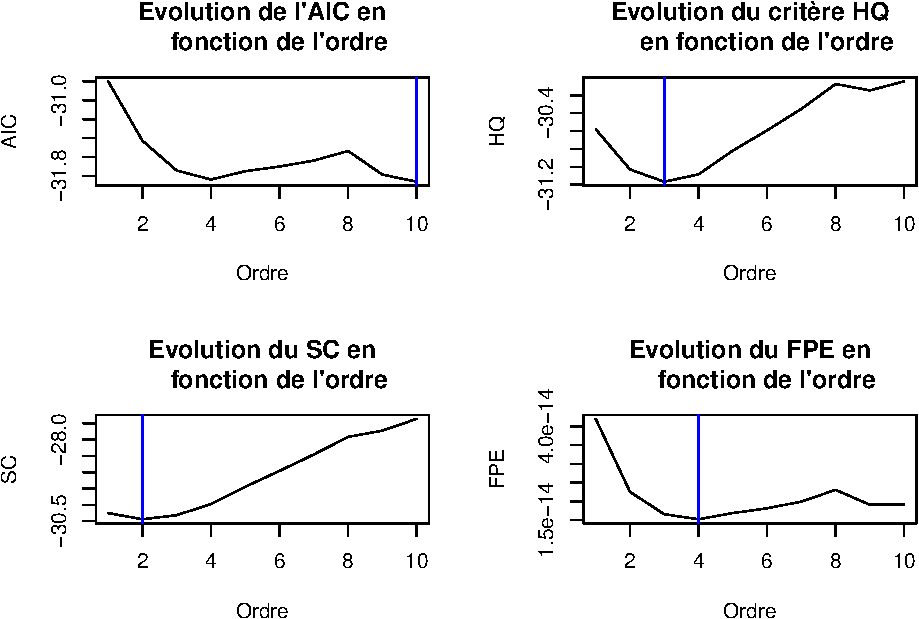
\includegraphics{doc_files/figure-latex/unnamed-chunk-10-1.pdf}

On s'aperçoit que les différents critères à notre disposition nous
donnent des ordres à choisir différents. Ainsi, le meilleur AIC
correspond à un modèle d'ordre 10, le meilleur HQ à un modèle d'ordre 3
et le meilleur SC à un modèle d'ordre 2. L'ordre de l'AIC étant trop
grand (car trop de coefficients à estimer par rapport au nombre
d'observations à notre disposition), nous ne souhaitons pas conserver
cet ordre. De plus, on se rend compte que l'AIC du modèle avec un ordre
10 est similaire à celle d'un modèle avec un ordre 4. Les modèles HQ et
SC sont meilleurs avec respectivement un ordre 3 et 2. Nous allons donc,
dans la suite de l'analyse, veillez à minimiser le critère AIC, tout en
étant attentif aux autres critères. C'est pourquoi, ici, nous décidons
de conserver un ordre 4.

\section{Estimation du modèle}\label{estimation-du-modele}

Dans la partie précédente, nous avons sélectionné le meilleur ordre pour
notre modèle VAR. Il s'agit maintenant d'estimer différents modèles afin
de pouvoir prédire la MSE. L'exemple que nous avons pris est pour le
modèle complet, qui nous donne donc un ordre de 4.

Un modèle VAR s'écrit sous la forme suivante.:

\(y_t = \sum_{i = 1}^{p} {A_iy_{t-i}} + u_t\)

\(A_i\) représentent les matrices de coefficients du modèle pour un
ordre i, t le décalage de la série et \(u_t\) le vecteur des résidus.
Dans notre cas, nous aurons donc 3 matrices de taille 5x5.

Dans le package \textbf{vars}, la fonction utilisée pour construire des
modèles VAR est VAR, qui prend en entrée la série temporelle
multivariée, l'ordre du processus et le type de régresseurs à inclure.
Dans notre cas, \emph{type} vaut \emph{const} car la série est
stationnarisée et donc centrée en une constante \(\mu\).

\begin{Shaded}
\begin{Highlighting}[]
\NormalTok{modele<-}\KeywordTok{VAR}\NormalTok{(}\KeywordTok{cbind}\NormalTok{(MSEStaTrain, PIBStaTrain, SMICStaTrain, TCHOFStaTrain), }\DataTypeTok{p=}\DecValTok{4}\NormalTok{, }\DataTypeTok{type=}\StringTok{"const"}\NormalTok{)}
\end{Highlighting}
\end{Shaded}

Les coefficients du modèle sont les suivants

\begin{Shaded}
\begin{Highlighting}[]
\NormalTok{A1<-}\KeywordTok{cbind}\NormalTok{(modele$varresult$MSEStaTrain$coefficients[}\DecValTok{1}\NormalTok{:}\DecValTok{4}\NormalTok{], }
          \NormalTok{modele$varresult$PIBStaTrain$coefficients[}\DecValTok{1}\NormalTok{:}\DecValTok{4}\NormalTok{], }
          \NormalTok{modele$varresult$SMICStaTrain$coefficients[}\DecValTok{1}\NormalTok{:}\DecValTok{4}\NormalTok{],}
          \NormalTok{modele$varresult$TCHOFStaTrain$coefficients[}\DecValTok{1}\NormalTok{:}\DecValTok{4}\NormalTok{])}
\KeywordTok{colnames}\NormalTok{(A1)<-}\KeywordTok{rownames}\NormalTok{(A1)<-}\KeywordTok{c}\NormalTok{(}\StringTok{"MSE"}\NormalTok{, }\StringTok{"PIB"}\NormalTok{, }\StringTok{"SMIC"}\NormalTok{, }\StringTok{"TCHOF"}\NormalTok{)}
\NormalTok{A1}
\end{Highlighting}
\end{Shaded}

\begin{verbatim}
##               MSE           PIB        SMIC      TCHOF
## MSE   -0.49912624 -0.0308097020  0.05328488 -0.8445102
## PIB    0.92777848  0.1257671971  1.21484663 -5.9314489
## SMIC   0.06599595 -0.0051246390 -0.49802200  0.6626694
## TCHOF -0.01352986  0.0006699293 -0.01008137 -0.3235506
\end{verbatim}

Dans cette fonction, nous ne disposons pas des erreurs standards
associées aux coefficients. Les indicateurs de qualité du modèle sont
présents ci-dessous.

\begin{Shaded}
\begin{Highlighting}[]
\NormalTok{selection<-}\KeywordTok{VARselect}\NormalTok{(}\KeywordTok{cbind}\NormalTok{(MSEStaTrain, PIBStaTrain, SMICStaTrain, TCHOFStaTrain))}
\NormalTok{selection$criteria[,}\DecValTok{4}\NormalTok{]}
\end{Highlighting}
\end{Shaded}

\begin{verbatim}
##        AIC(n)         HQ(n)         SC(n)        FPE(n) 
## -3.183609e+01 -3.108380e+01 -2.997216e+01  1.517819e-14
\end{verbatim}

\section{Prévisions}\label{previsions}

Maintenant que nous avons estimé l'ordre des différents modèle VAR, et
que nous avons explicité l'estimation des modèles, nous cherchons
désormais à trouver celui dont les prédictions sont les plus proches de
la réalité.

Après avoir comparé tous les modèles possibles (7 : 3 modèles avec deux
variables, 3 modèles avec trois variables et un modèle avec les quatre
variables), nous nous apercevons que le meilleur en terme de prédictions
est le modèle prenant en compte le SMIC (en plus de la masse salariale).

\begin{Shaded}
\begin{Highlighting}[]
\CommentTok{#SMIC}
\KeywordTok{VARselect}\NormalTok{(}\KeywordTok{cbind}\NormalTok{(MSEStaTrain, SMICStaTrain), }\DataTypeTok{lag.max=}\DecValTok{10}\NormalTok{)}
\end{Highlighting}
\end{Shaded}

\begin{verbatim}
## $selection
## AIC(n)  HQ(n)  SC(n) FPE(n) 
##      3      3      3      3 
## 
## $criteria
##                    1             2             3             4
## AIC(n) -1.437706e+01 -1.504929e+01 -1.541342e+01 -1.538725e+01
## HQ(n)  -1.431068e+01 -1.493865e+01 -1.525853e+01 -1.518811e+01
## SC(n)  -1.421259e+01 -1.477518e+01 -1.502967e+01 -1.489386e+01
## FPE(n)  5.703539e-07  2.912536e-07  2.024391e-07  2.079440e-07
##                    5             6             7             8
## AIC(n) -1.535114e+01 -1.530767e+01 -1.535484e+01 -1.529623e+01
## HQ(n)  -1.510775e+01 -1.502003e+01 -1.502295e+01 -1.492008e+01
## SC(n)  -1.474810e+01 -1.459500e+01 -1.453252e+01 -1.436427e+01
## FPE(n)  2.158164e-07  2.257434e-07  2.157878e-07  2.294353e-07
##                    9            10
## AIC(n) -1.525746e+01 -1.526620e+01
## HQ(n)  -1.483706e+01 -1.480155e+01
## SC(n)  -1.421586e+01 -1.411495e+01
## FPE(n)  2.393329e-07  2.382777e-07
\end{verbatim}

\begin{Shaded}
\begin{Highlighting}[]
\KeywordTok{VAR}\NormalTok{(}\KeywordTok{cbind}\NormalTok{(MSEStaTrain, SMICStaTrain), }\DataTypeTok{p=}\DecValTok{3}\NormalTok{, }\DataTypeTok{type=}\StringTok{"const"}\NormalTok{)}
\end{Highlighting}
\end{Shaded}

\begin{verbatim}
## 
## VAR Estimation Results:
## ======================= 
## 
## Estimated coefficients for equation MSEStaTrain: 
## ================================================ 
## Call:
## MSEStaTrain = MSEStaTrain.l1 + SMICStaTrain.l1 + MSEStaTrain.l2 + SMICStaTrain.l2 + MSEStaTrain.l3 + SMICStaTrain.l3 + const 
## 
##  MSEStaTrain.l1 SMICStaTrain.l1  MSEStaTrain.l2 SMICStaTrain.l2 
##    -0.554842568     0.001362944    -0.550136180    -0.014196261 
##  MSEStaTrain.l3 SMICStaTrain.l3           const 
##    -0.395923428    -0.013169066     2.500225678 
## 
## 
## Estimated coefficients for equation SMICStaTrain: 
## ================================================= 
## Call:
## SMICStaTrain = MSEStaTrain.l1 + SMICStaTrain.l1 + MSEStaTrain.l2 + SMICStaTrain.l2 + MSEStaTrain.l3 + SMICStaTrain.l3 + const 
## 
##  MSEStaTrain.l1 SMICStaTrain.l1  MSEStaTrain.l2 SMICStaTrain.l2 
##     -0.01867915     -0.54580898     -0.22996141     -0.74042266 
##  MSEStaTrain.l3 SMICStaTrain.l3           const 
##     -0.35846413     -0.46120378      0.60780380
\end{verbatim}

\begin{Shaded}
\begin{Highlighting}[]
\NormalTok{VARSMICSta <-}\StringTok{ }\KeywordTok{forecast}\NormalTok{(}\KeywordTok{VAR}\NormalTok{(}\KeywordTok{cbind}\NormalTok{(MSEStaTrain, SMICStaTrain), }\DataTypeTok{p=}\DecValTok{3}\NormalTok{, }\DataTypeTok{type=}\StringTok{"const"}\NormalTok{))}
\KeywordTok{plot}\NormalTok{(MSETest, }\DataTypeTok{xlim=}\KeywordTok{c}\NormalTok{(}\DecValTok{2016}\NormalTok{,}\FloatTok{2016.75}\NormalTok{), }\DataTypeTok{main=}\StringTok{"Différences entre les véritables}
\StringTok{     valeurs de 2016 et les prédictions du modèle pour la masse salariale"}\NormalTok{)}
\CommentTok{#Reconstruction de la variable stationnaire}
\NormalTok{recon <-}\StringTok{ }\NormalTok{VARSMICSta$forecast$MSEStaTrain$mean *}\StringTok{ }\NormalTok{MSETrendTest *}\StringTok{ }\NormalTok{MSESeasonalTest}
\KeywordTok{lines}\NormalTok{(recon, }\DataTypeTok{col =} \StringTok{"red"}\NormalTok{)}
\KeywordTok{legend}\NormalTok{(}\StringTok{'bottomleft'}\NormalTok{, }\DataTypeTok{legend =} \KeywordTok{c}\NormalTok{(}\StringTok{'Vraies valeurs'}\NormalTok{, }\StringTok{'Prévisions du modèle'}\NormalTok{),}
       \DataTypeTok{col=}\KeywordTok{c}\NormalTok{(}\StringTok{'black'}\NormalTok{, }\StringTok{'red'}\NormalTok{), }\DataTypeTok{lty=}\DecValTok{1}\NormalTok{, }\DataTypeTok{cex=}\FloatTok{0.8}\NormalTok{)}
\end{Highlighting}
\end{Shaded}

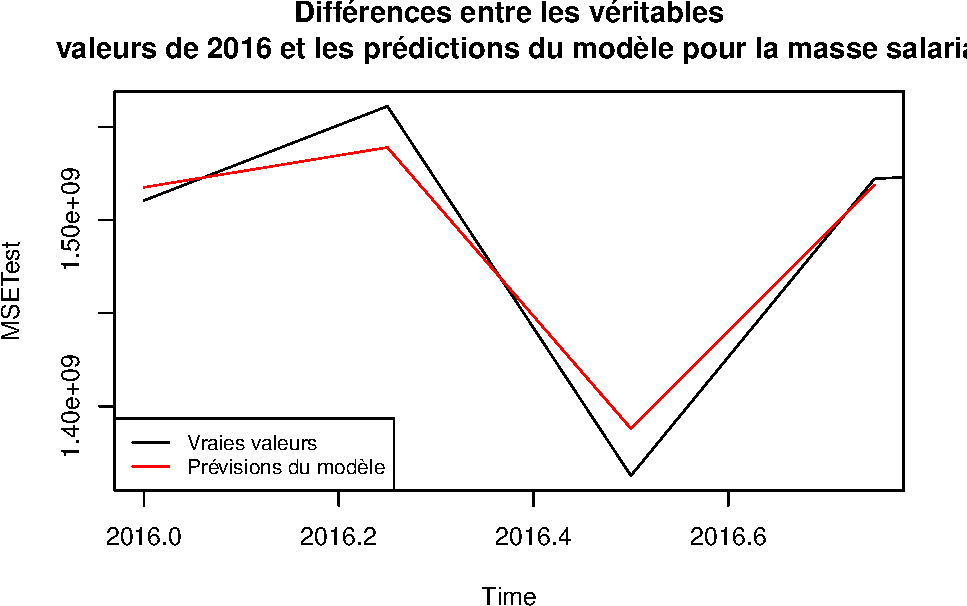
\includegraphics{doc_files/figure-latex/unnamed-chunk-14-1.pdf}

Nous nous intéressons donc à l'erreur quadratique moyenne de cette
prévision.

\begin{Shaded}
\begin{Highlighting}[]
\KeywordTok{EQM}\NormalTok{(MSETest, recon)}
\end{Highlighting}
\end{Shaded}

\begin{verbatim}
## [1] 1.984486e+14
\end{verbatim}


\end{document}
